\begin{figure}[h!]
    \centering
    \caption{Average rent, square footage, and rent per square footage by (residualized) household income decile}
    \label{fig:ahs_rent_sqft}

    \begin{subfigure}{.49\textwidth}
        \caption{Average residualized rent}
        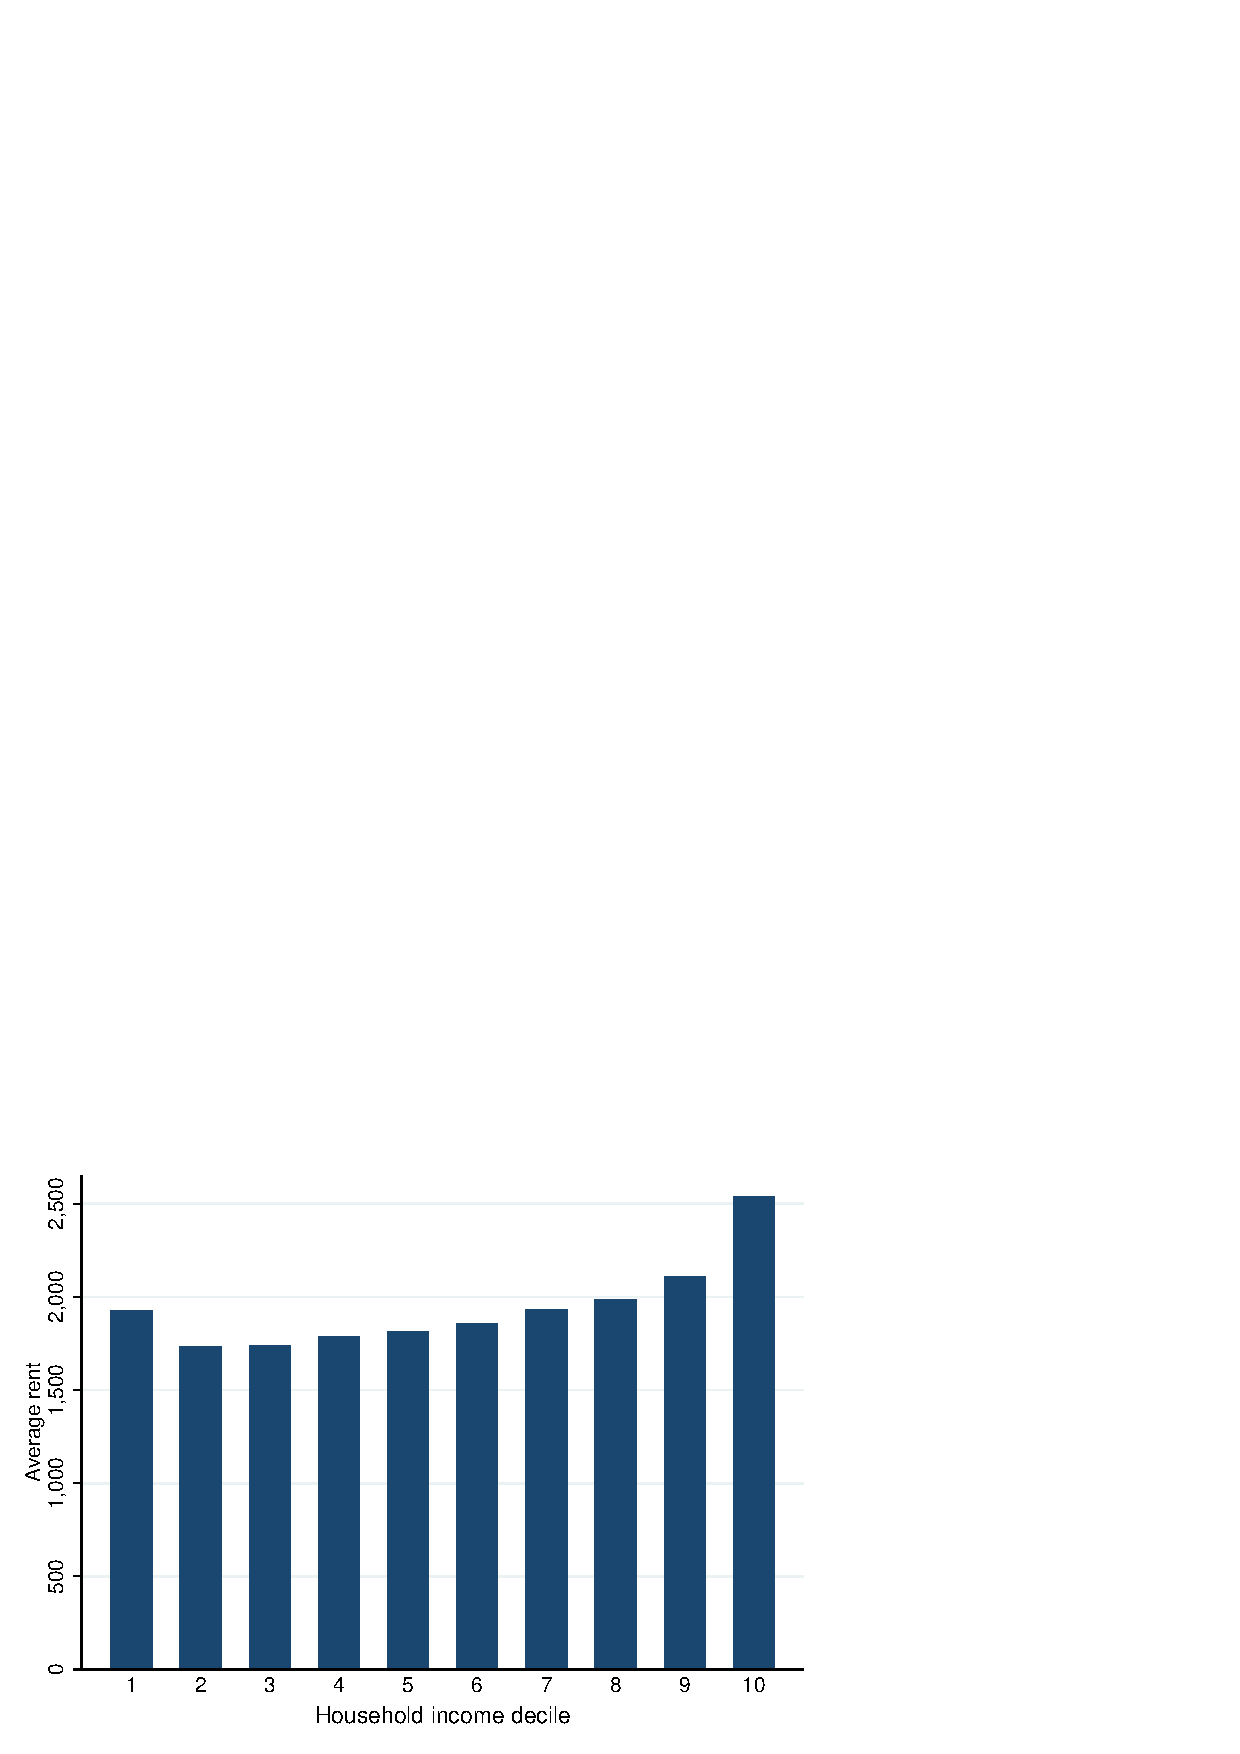
\includegraphics[width = 1\textwidth]
            {ahs/output/avg_rent}
    \end{subfigure}%
    \begin{subfigure}{.49\textwidth}
        \caption{Average residualized square footage}
        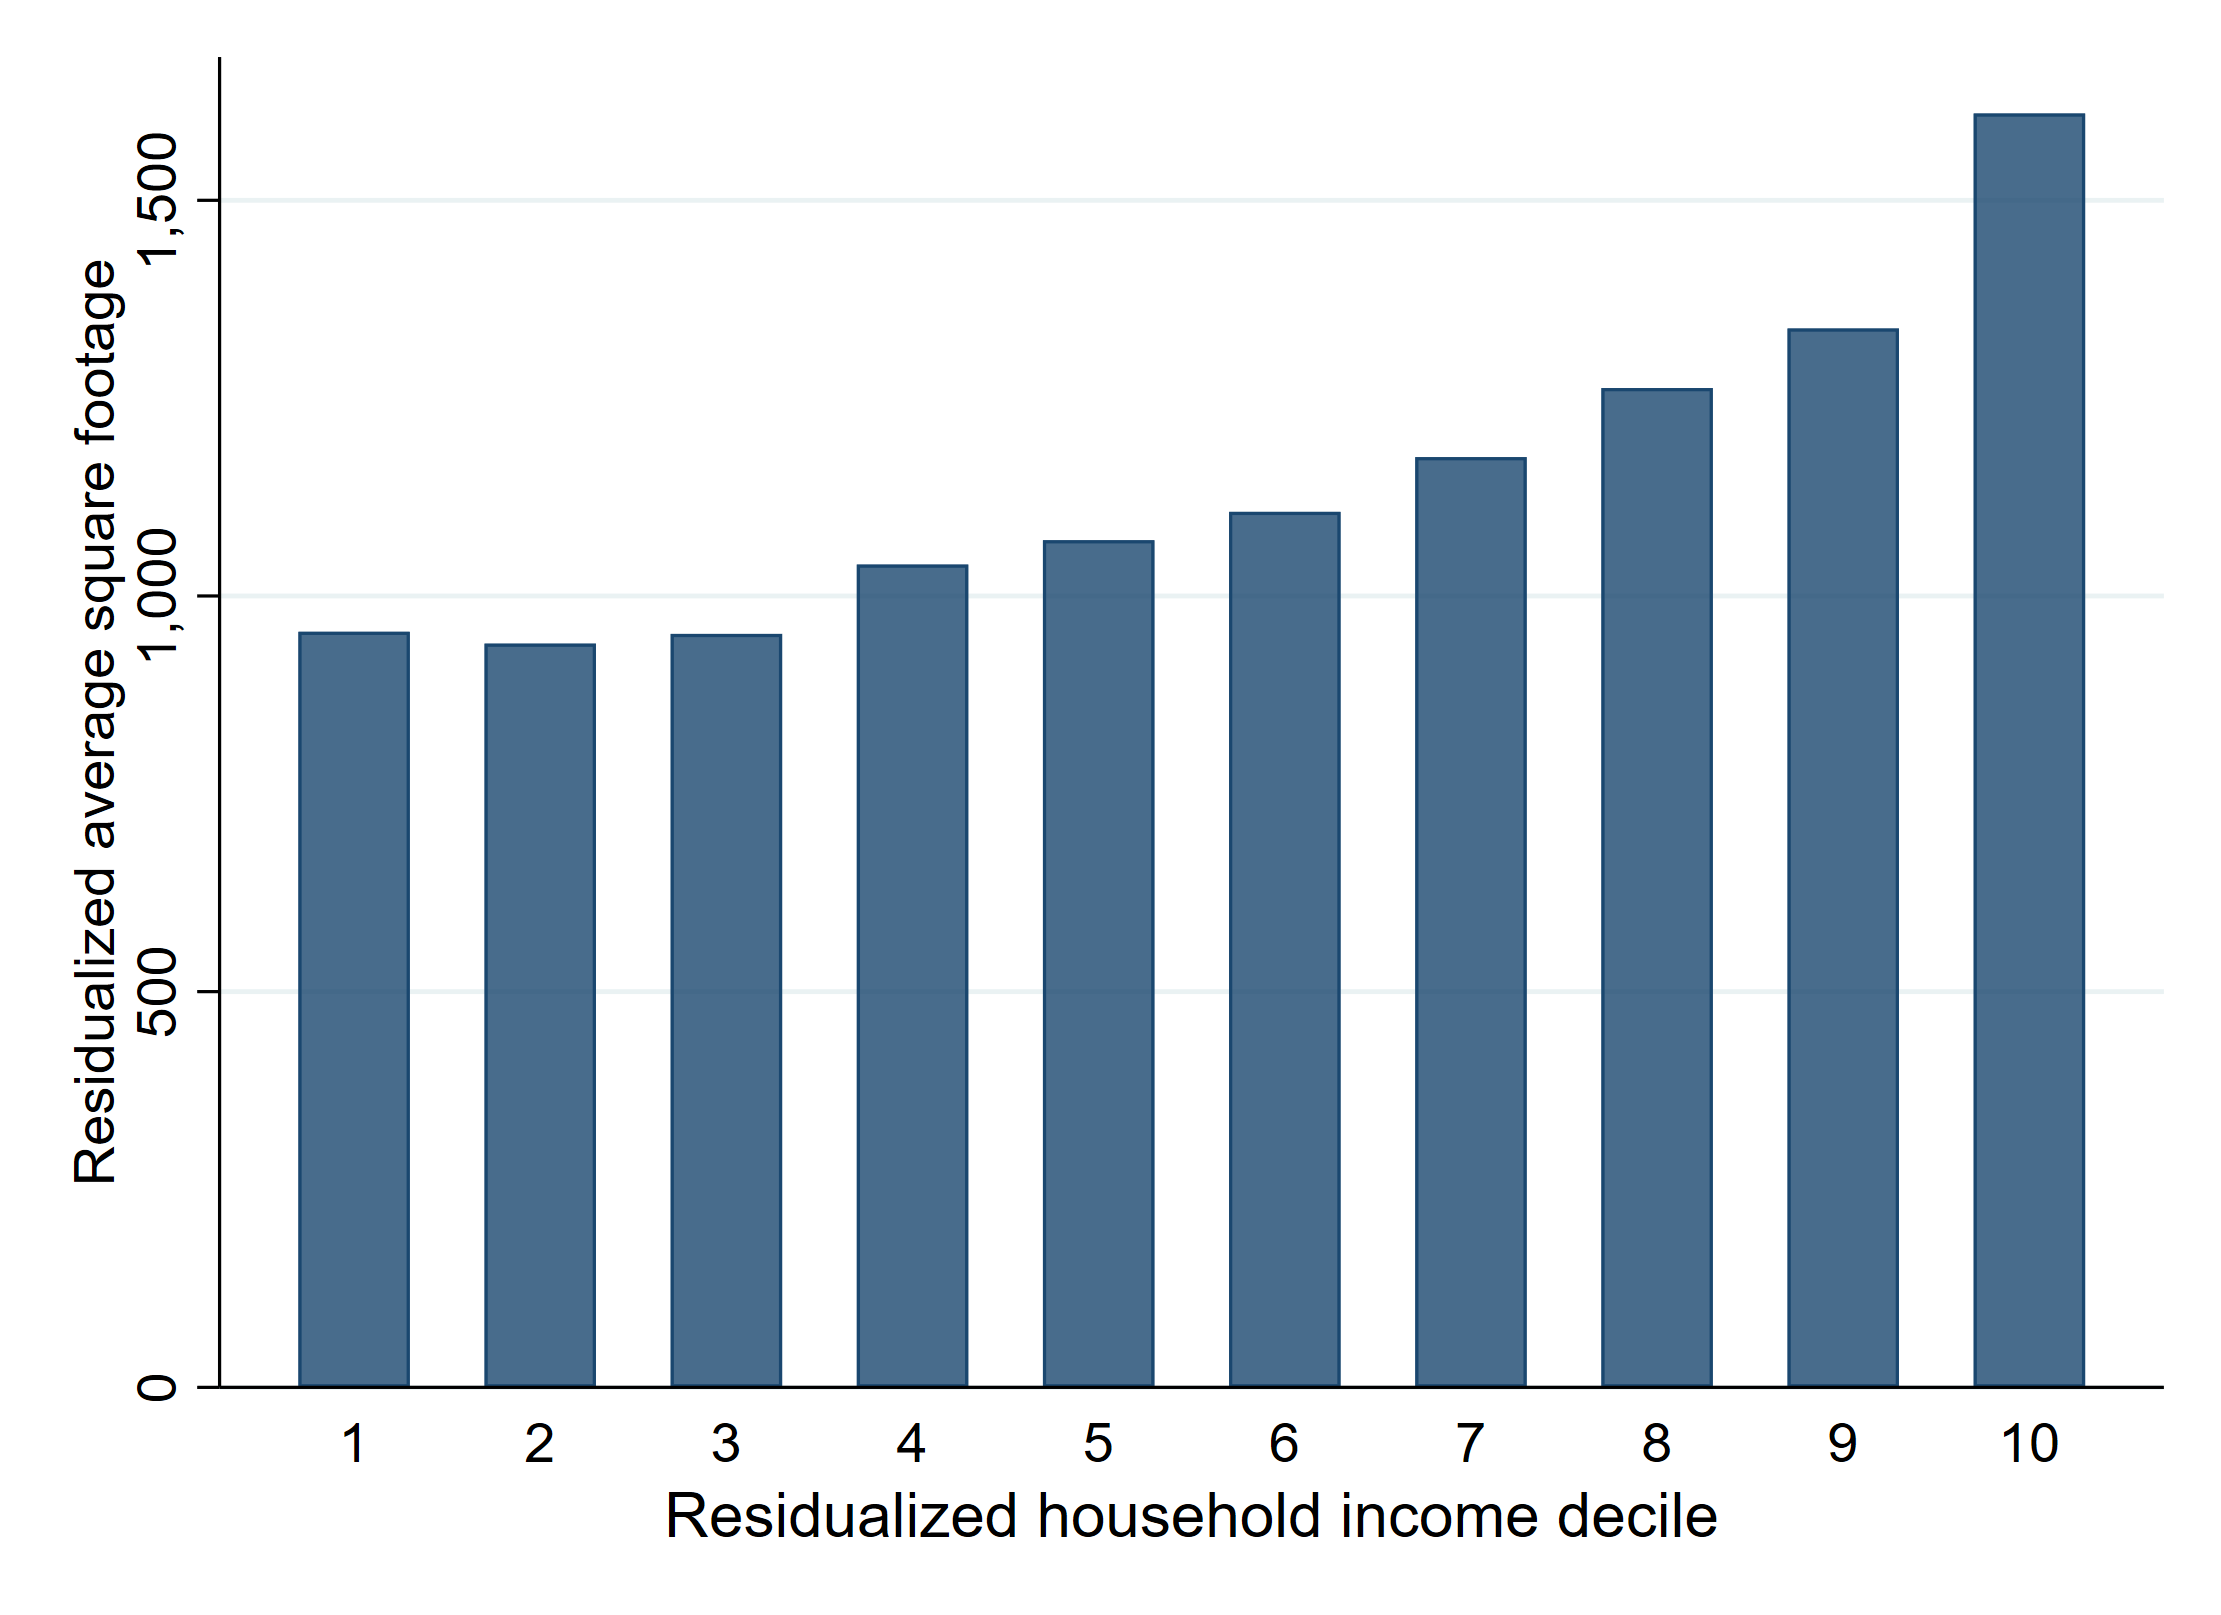
\includegraphics[width = 1\textwidth]
            {ahs/output/avg_sqft}
    \end{subfigure}\\
    \begin{subfigure}{.67\textwidth}
        \caption{Average residualized rent per square footage}
        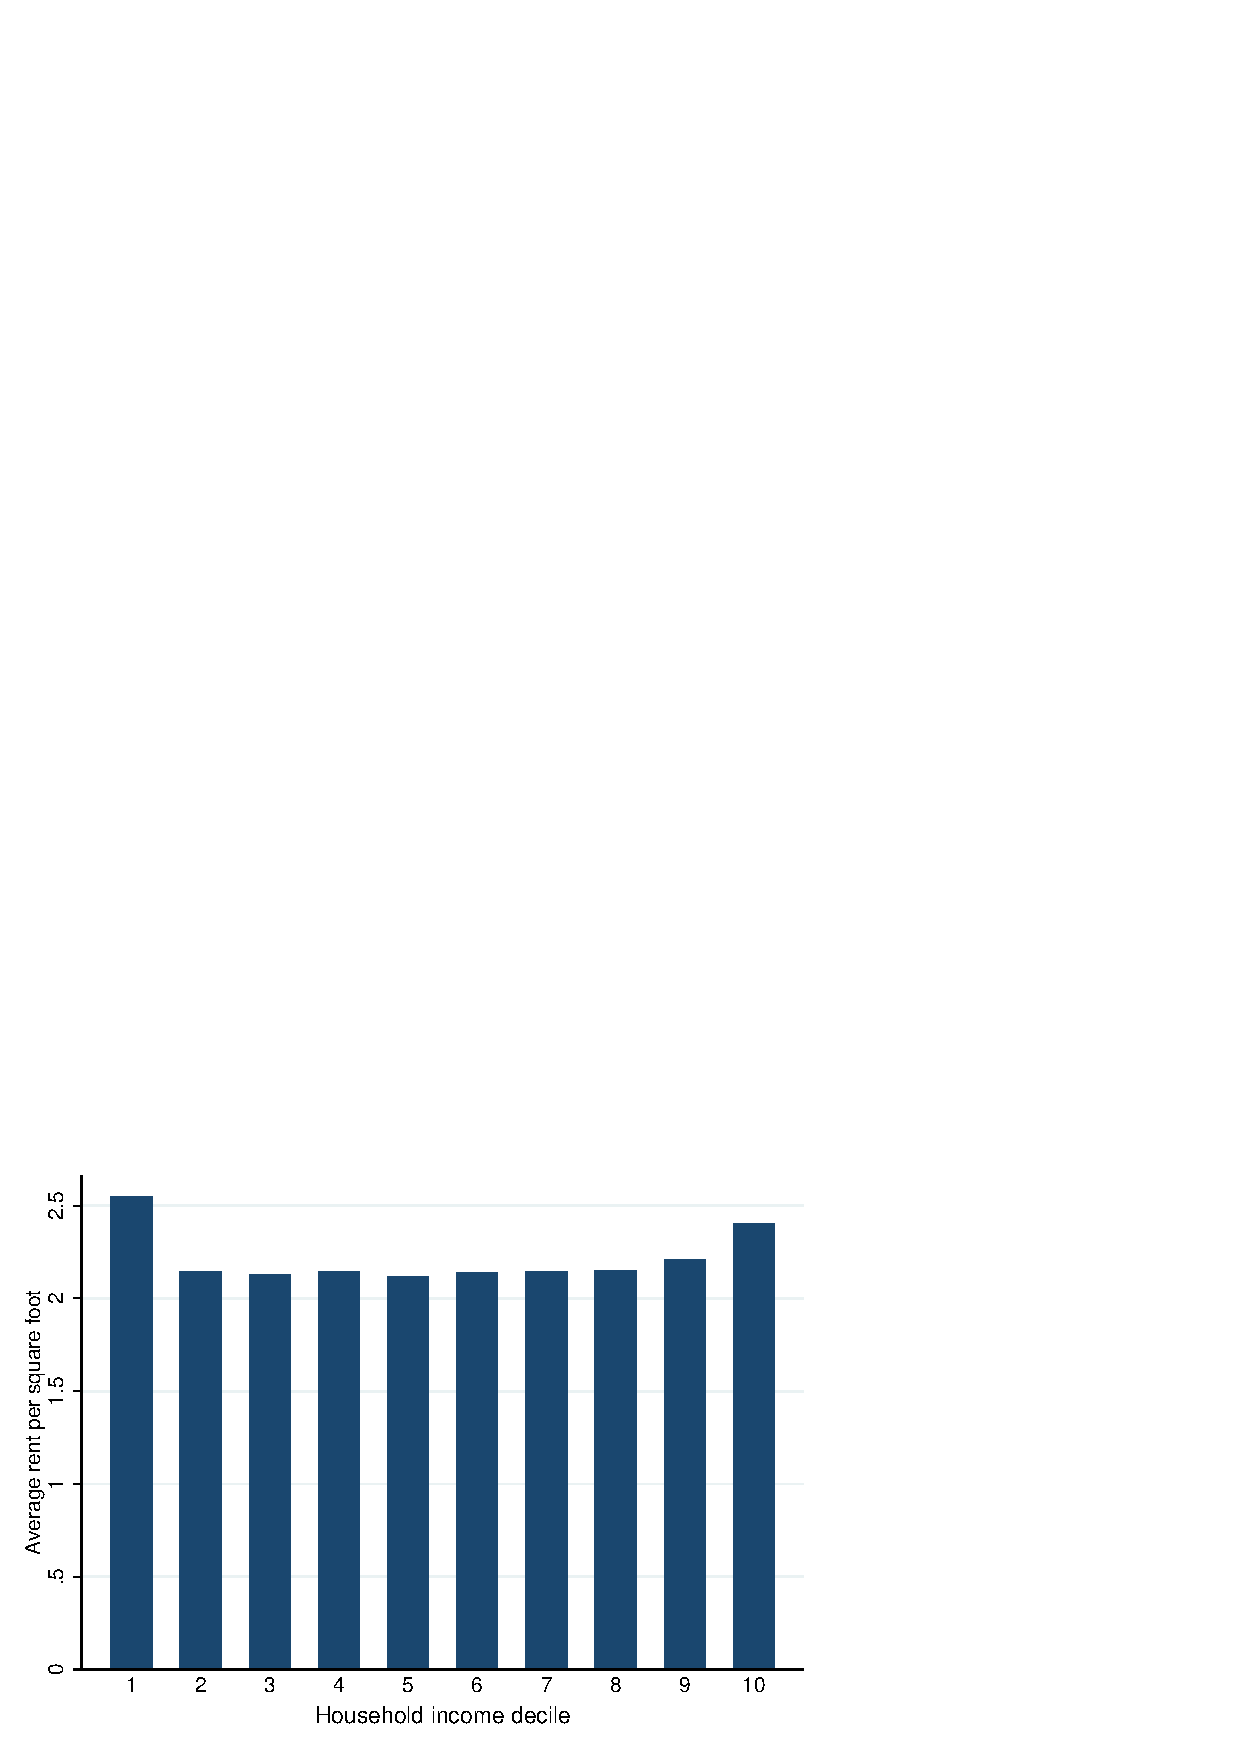
\includegraphics[width = 1\textwidth]
            {ahs/output/avg_rent_psqft}
    \end{subfigure}

    \begin{minipage}{.95\textwidth} \footnotesize
        \vspace{3mm}
        Notes: Data are from the 2011 and 2013 American Housing
        Survey (AHS), as described in Section \ref{ADD SECTION}. 
        The top left figure shows the average rent by household 
        income, the top right figure shows the average square 
        footage by household income, and the bottom figure shows
        the average rent per square footage by household income.
        All of the variables are residualized at the SMSA level.
        We exclude from the calculation non-conventional housing units, 
        such as mobile homes, hotels, rooming houses, etc.
    \end{minipage}
\end{figure}
